%!TEX root = ../rapport.tex
%!TEX encoding = UTF-8 Unicode

% Chapitres "Introduction"

% modifié par Francis Valois, Université Laval
% 31/01/2011 - version 1.0 - Création du document

\chapter{Avancements pratiques}
\label{s:avancement}
Cette section décrit les avancements dans la conception et dans la construction du système Kinocto.
\section{Alimentation des périphériques 5V}
L'alimentation employée pour les périphériques est une alimentation de type buck qui convertit la tension de la batterie (11.1V) vers une tension usuelle de 5V. Cette alimentation utilise un hacheur de tension avec une fréquence autour de 50kHz. Cette fréquence procure une marge de sécurité par rapport à la fréquence d'antenne et évite l'ajout d'un bruit excessif. Cette alimentation a été réalisée avec succès, les plans sont présentés à la figure \ref{fig:alim5V}. Une photo de ladite alimentation est présentée à la figure \ref{fig:alim5Vphoto}.

\begin{figure}[htbp]
\centering
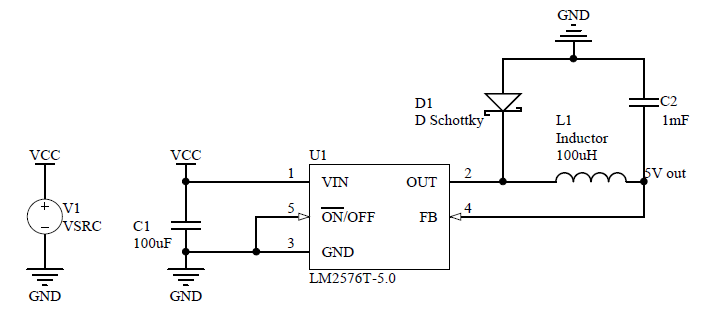
\includegraphics[scale=0.5]{fig/alim_5V.png}
\caption{Figure présentant les plans de l'alimentation 5V pour les périphériques}
\label{fig:alim5V}
\end{figure}

\begin{figure}[htbp]
\centering
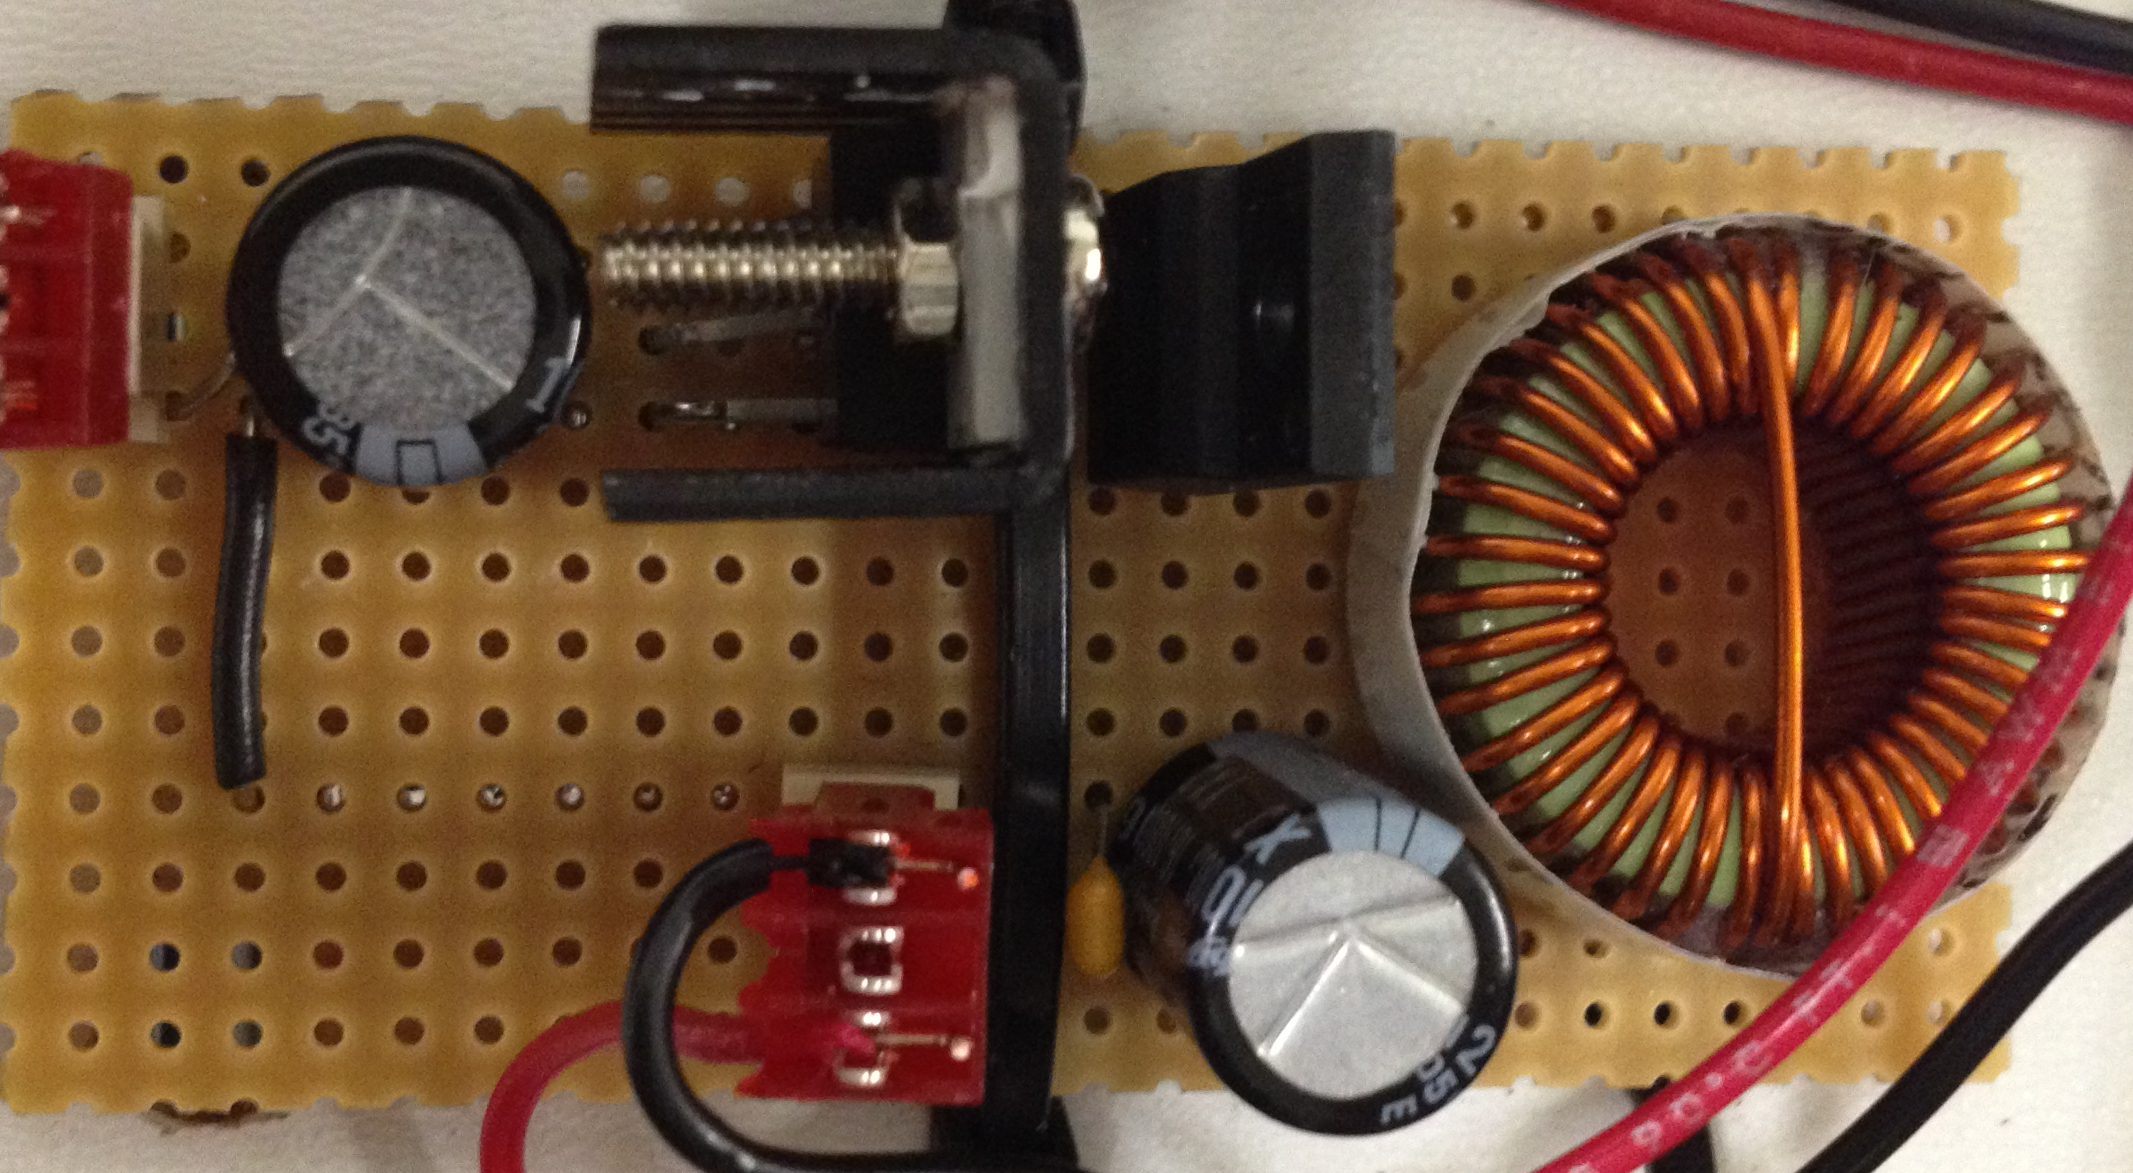
\includegraphics[scale=0.2]{fig/alim_5V_photo.png}
\caption{Figure présentant une photo de l'alimentation 5V pour les périphériques}
\label{fig:alim5Vphoto}
\end{figure}

\section{Alimentation 24V du Mac mini et du préhenseur}
Le Mac mini et le préhenseur sont alimentés avec une tension de 24V. Une alimentation correspondante a été achetée déjà préconçue et préassemblée sur circuit imprimé. Cette solution représente le choix de design le plus économique et le plus fiable selon nos hypothèses. Ce module est un hacheur survolteur dans lequel la tension de 11.1V de la batterie est ammenée à 24V. Le rendement obtenu est d’environ 94\% et les ondulations de tensions sont considérées comme négligeables. \ref{fig:alim24Vphoto}.

\begin{figure}[htbp]
\centering
\includegraphics[scale=0.1]{fig/alim_24V_photo.png}
\caption{Figure présentant une photo de l'alimentation 24V pour les périphériques}
\label{fig:alim24Vphoto}
\end{figure}

\section{Réception du signal Manchester}
Pour la réception du signal Manchester est réalisée au moyen d'un circuit intégré de décodage de tonalité, le LM567. Ce circuit intégré met de sortie à la masse lorsqu’il détecte la fréquence ciblée sur son entrée. Le signal d'antenne recueilli par le décodeur est capté par un fil bobiné sur plusieurs tours autour du préhenseur (voir la figure \ref{fig:prehenseur2}). L'augmentation du nombre de tours de fil permet de maximiser les variations de flux magnétique.  Un comparateur à hystérésis est utilisé à la sortie du décodeur afin de contourner les variations de tension causées par l'intensité variable du signal d’entrée. Cependant, comme le signal de sortie du décodeur est inversé, la sortie du comparateur passe dans un inverseur et est envoyée ensuite dans le microcontrôleur qui le décode. Ce récepteur est opérationnel depuis quelques semaines déjà. Le plan de ce récepteur est présenté à la figure \ref{fig:manchester}.

\begin{figure}[htbp]
\centering
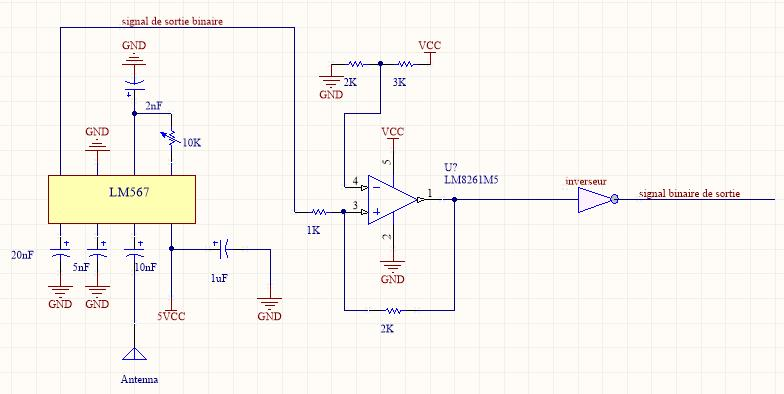
\includegraphics[scale=0.5]{fig/circuit_manchester.jpg}
\caption{Figure présentant les plans du récepteur manchester}
\label{fig:manchester}
\end{figure}

\section{Préhenseur}
Le préhenseur est réalisé à l’aide d’un actionneur magnétique qui reçoit une commande de 0V ou de 5V qui lui indique s’il doit abaisser ou remonter le crayon. Le circuit magnétique exerce une force vers le bas sur le crayon lorsque la commande est à 5V. Un élastique permet le retour en place du crayon. Pour minimiser les points morts lors des changements de direction du robot, un système de plongeur qui progresse dans un guide à faible tolérance est utilisé. La présence du guide maximise la précision de l’actionneur magnétique (l'angle du crayon reste constant). Le préhenseur est actionné à partir d'une commande analogique 0-5V fournie par le microcontrôleur. Ce signal est injecté sur la gâchette d’un transistor MOSFET qui commute la tension 24V issue de la batterie sur l'entrée du préhenseur. Le préhenseur et son système de commande sont opérationnels depuis un certain temps déjà. On peut observer le schéma du circuit de commande du préhenseur sur la figure \ref{fig:prehenseur} ainsi que sa réalisation mécanique sur la figure \ref{fig:prehenseur2}.

\begin{figure}[htbp]
\centering
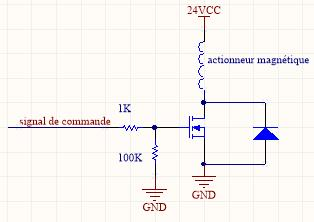
\includegraphics[scale=0.5]{fig/prehenseur.jpg}
\caption{Figure présentant les plans du circuit de commande du préhenseur}
\label{fig:prehenseur}
\end{figure}

\begin{figure}[htbp]
\centering
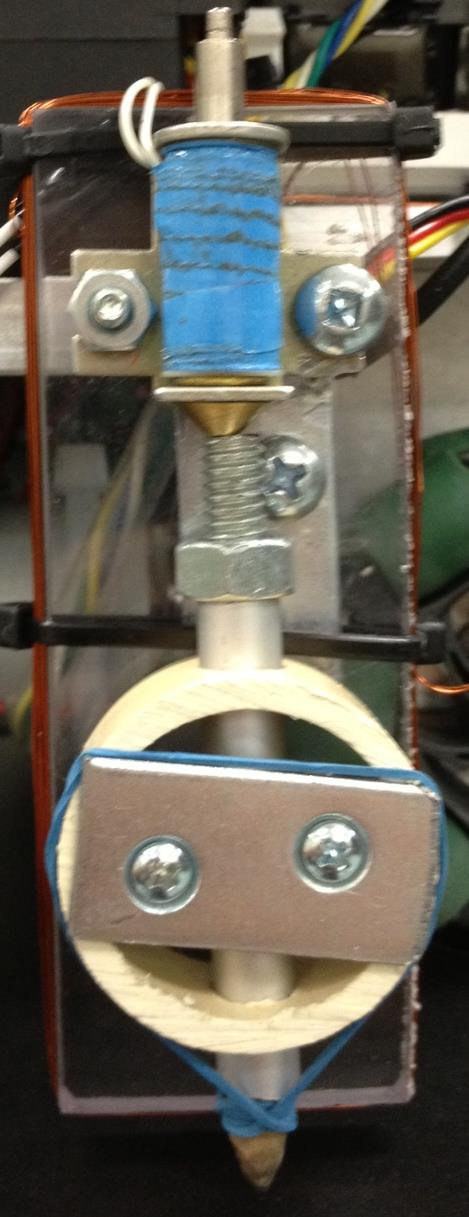
\includegraphics[scale=0.5]{fig/prehenseur2.jpg}
\caption{Figure présentant la réalisation mécanique du préhenseur}
\label{fig:prehenseur2}
\end{figure}

\section{DEL verte de fin de tâche}
Pour le circuit de la DEL verte qui confirme la fin des tâches du robot, un transistor MOSFET de faible puissance est utilisé. Il reçoit un signal analogique de commande du microcontrôleur sur sa grille et commute une tension de 5V aux bornes de la DEL. Le circuit est présenté à la figure \ref{fig:del_verte}.

\begin{figure}[htbp]
\centering
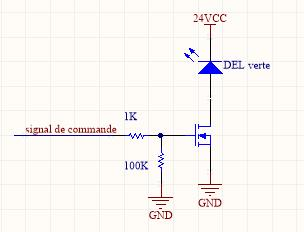
\includegraphics[scale=0.5]{fig/del_verte.jpg}
\caption{Figure présentant les plans du circuit de commande du préhenseur}
\label{fig:del_verte}
\end{figure}

\section{Circuit de protection}
Pour le circuit de protection, trois fusibles en série avec des interrupteurs ont été employés pour alimenter chacun des circuits d’alimentation 11,1V, 5V et 24V. Chacun des interrupteurs est muni d’un témoin lumineux qui confirme sa mise sous tension et valide que son fusible soit intact.

\section{Source d'énergie}
Pour alimenter les différents composants du robot, une batterie lithium-polymère, connue pour sa grande capacité énergétique par unité de volume, est utilisée. La pile employée comporte 3 cellules en série et produit une tension totale de 11.1V pour une capacité totale de 5Ah. Une telle capacité permet une autonomie de 30 minutes dans le pire des cas.


\section{Asservissement des moteurs}
\subsection{Modélisation}
L'optimisation des paramètres de réglage a été réalisée grâce à l'utilisation d'un outil de CAO élaboré au moyen de Matlab-Simulink. La fonction de transfert des moteurs a été identifiée au moyen d'une réponse à l'échelon et de l'outil \textit{ident} de Matlab. L'ordre choisi de la fonction est élevé et présente une concordance de 94\% avec la réponse obtenue expérimentalement. L'outil \textit{pidtool} permet par la suite de configurer adéquatement le PIDF et d'obtenir la réponse souhaitée et les paramètres associés. Suivant ces paramètres, le PIDF présent dans le microcontrôleur est ajusté.
\paragraph{}L'usage de l'outil interactif permet d'optimiser la réponse et d'obtenir des paramètres de préréglages qui limitent le nombre d'itérations. La réponse obtenue logiciellement est présentée à la figure \ref{fig:as_1}
\begin{figure}[htbp]
\centering
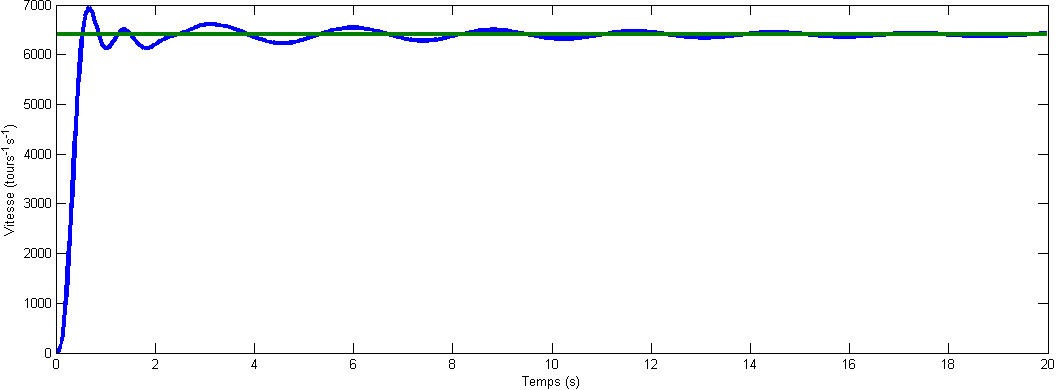
\includegraphics[scale=0.6]{fig/asservissement_1.png}
\caption{Figure présentant la réponse à un échelon de consigne de 6400$\left[tours^{-1}s^{-1}\right]$ du système régulé au moyen du régulateur optimisé dans simulink}
\label{fig:as_1}
\end{figure}
\subsection{Implantation pratique}
\label{s:ass_implantation_pratique}
La réponse à un échelon de consigne de 6400 ($tours^{-1} s^{-1}$) avec les paramètres de réglage réels est présentée à la figure \ref{fig:as_2}. À noter que les consignes en $tours^{-1} s^{-1}$ indiquent la vitesse en nombre de 1/6400 de tours de roue. Cette fraction de tour est due au fait que les interfaces d'encodeurs en quadratures captent 6400 transitions par tour complet de roue (voir la sous-section \ref{asservissement_mesures} pour plus de détails).
Le système a été implanté avec un asservissement en vitesse et sans asservissement de position. Les expériences pratiques réalisées montrent que l'évolution de la position est linéaire, et ce, sans asservissement. La figure \ref{fig:as_3} présente ce phénomène pour une consigne de 6400 ($tours^{-1} s^{-1}$) qui vise à amener le système à une position de 9100 $tours^{-1}$.
En utilisant les paramètres obtenus dans Matlab comme point de départ, les paramètres de réglages ont été modifiés de manière à obtenir des réponses remplissant les critères de stabilité, de vitesse et de dépassement souhaités. Afin d'améliorer la vitesse des déplacements, différents PID ont été ajustés selon différentes vitesses d'asservissement. On compte trois de ces PID pour les déplacements unilatéraux et un réservé pour les mouvements reliés au dessin. La différence est que la vitesse de dessin est beaucoup plus basse que celle du déplacement usuel en vue de permettre une plus grande précision. Le moteur n'est plus linéaire à de faibles vitesses (roulement et zone morte très limitants) et le système est incapable de démarrer de lui-même, Il est donc impossible, pour de faibles vitesses, de procéder avec une modélisation linéaire du système. Le PID a donc été ajusté de manière manuelle, par itérations. Les PID sont fonctionnels et les systèmes stables, cependant, la décélération avant l'arrêt et le positionnement critique se font par l'entremise d'un palier de ralentissement à une vitesse intermédiaire avant freinage. Ces courbes de décélérations sont à mettre au point avant de pouvoir entamer le contrôle en dessin. Par ailleurs, les mouvements en diagonale ne sont pas encore parfaitement au point et requièrent quelques heures de travail additionnelles.
\begin{figure}[htbp]
\centering
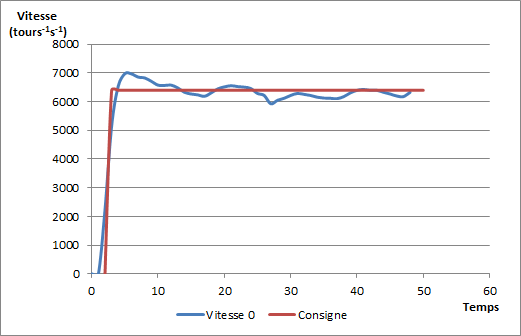
\includegraphics[scale=0.6]{fig/asservissement_3.png}
\caption{Figure présentant la réponse à un échelon de consigne de 6400$\left[tours^{-1}s^{-1}\right]$ du système régulé au moyen du régulateur réel et de la réponse en position associée}
\label{fig:as_2}
\end{figure}
\begin{figure}[htbp]
\centering
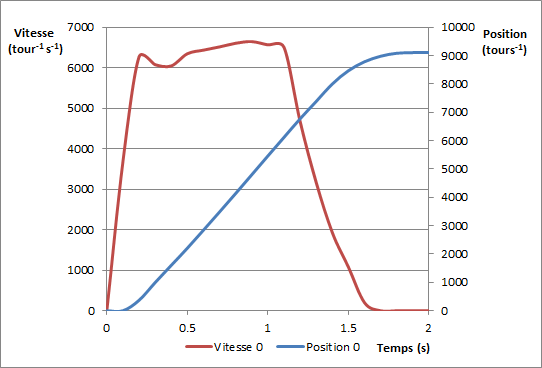
\includegraphics[scale=0.6]{fig/asservissement_2.png}
\caption{Figure présentant la réponse à un échelon de consigne de 6400$\left[tours^{-1}s^{-1}\right]$ du système régulé au moyen du régulateur réel et de la réponse en position associée}
\label{fig:as_3}
\end{figure}
\subsection{Implantation électronique}
\subsubsection{Les prises de mesures}
\label{asservissement_mesures}
Deux QEI (Quadrature Encoder Interface) présents sur le microcontrôleur sont utilisés pour prendre des mesures de positions et de vitesses dans l'optique de fermer la boucle d'asservissement. Ces deux interfaces prennent en entrée les sorties des encodeurs situés sur les moteurs et captent les transitions lors de la rotation des moteurs. Puisqu'il y a deux capteurs placés en quadrature sur chaque moteur, on peut détecter la direction de la rotation des moteurs. À prendre note qu'un signal transmis par un encodeur contient 64 transitions par tour complet de moteur et que le ratio de la rotation moteur:roue est 100:1. Un signal transmis par un encodeur contient alors 6400 transitions pour une rotation complète de roue. Pour les deux autres moteurs, deux interfaces d'encodeurs en quadratures logicielles ont été réalisées à l'aide de deux broches d'entrées/sorties par interface, de courtes interruptions et d'une machine à états. Les interruptions sont lancées lorsqu'une transition est détectée sur l'une des broches. L'état des broches est alors lu et sauvegardé pour être traité par la machine à états. La machine à états utilisée est illustrée à la figure \ref{fig:cytron_machine_etats}. Les 0 et 1 indiqué dans les cercles identifient l'état logique des broches. Les -1 ou +1 tracés au dessus des transitions indiquent s'il faut incrémenter ou décrémenter la position de la roue en rotation.
\begin{figure}[htbp]
\centering
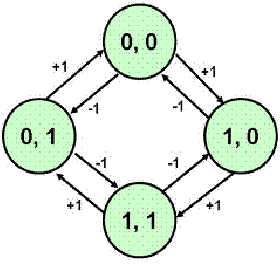
\includegraphics[scale=0.7]{fig/cytron_machine_etats.png}
\caption{Machine à états servant d'interface d'encodeur en quadrature (Cytron. Quadrature Encoder. \url{http://tutorial.cytron.com.my/2012/01/17/quadrature-encoder/}, consulté le 3 mars.)}
\label{fig:cytron_machine_etats}
\end{figure}
\subsubsection{PID}
Le PID utilisé pour l'asservissement est une courte fonction réalisée dans le microcontrôleur. La fonction théorique implémentée est présentée à l'équation \ref{eq:1}. Cette fonction se retrouve dans l'annexe \ref{s:fonction_PID}. Prendre note que l'argument "I" est le gain intégral de l'erreur et "dt" est le pas de temps. Cette fonction est exécutée individuellement pour chaque moteur. Des pointeurs transmis en argument indiquent l'emplacement en mémoire des valeurs de chaque moteur utilisées dans le PID. Ensuite, la fréquence d'exécution de la fonction est gardée constante à l'aide d'un timer dans le microcontrôleur qui déclenche une interruption à chaque période et lance l'exécution de l'asservissement.

\begin{equation}
\label{eq:1}
\mbox{PIDF}(z) = K_p + K_i \frac{T_s}{z-1} + K_d \frac{1}{T_f + \frac{T_s}{z -1}}
\end{equation}
Où
\begin{itemize}
\item $K_p$ est le gain proportionnel
\item $K_i$ est le gain intégral
\item $T_s$ est la durée d'un échantillon
\item $K_d$ est le gain différentiel
\item $T_f$ définit la coupure du filtre
\end{itemize}
\subsubsection{Ajustement de la vitesse selon la positon}
Comme indiqué précédemment, pour que le robot atteigne la consigne de position, la vitesse de la rotation des roues doit être ajustée selon la distance restante entre le robot et le point de destination. Cette ajustement est implanté par une simple multiplication d'un certain pourcentage avec la consigne de vitesse lorsque la distance restante à parcourir sera de "X" $tour^{-1}$. Le pourcentage utilisé présentement est hypothétique et sera ajusté lorsque les courbes de décélération discutées dans la section \ref{s:ass_implantation_pratique} seront identifiées.

\section{Servomoteurs de la Webcam}
Le contrôle des servomoteurs de la webcam est réalisé avec le contrôleur Micro Maestro de Pololu. L'application "Maestro Control Center" est employée afin de le programmer et de le configurer. Les servomoteurs et le Micro Maestro sont alimentés par l'alimentation 5V. De plus, ils reprennent une position prédéterminée lorsque ceux-ci et le Micro Maestro sont alimentés et restent fixes pour permettre à la Webcam de rester immobile même lorsque le robot est en mouvement. Prochainement, un script sera implanté dans le Micro Maestro à l'aide du "Maestro Control Center" pour transmettre par USB une commande du Mac mini au contrôleur un changement de position des servomoteurs. Cela a pour but de changer l'angle de la caméra web par rapport au sol. Ce changement est nécessaire afin de détecter l'orientation du robot.

\section{Extraction des sudocubes}
\subsection{Composantes du système}
L'algorithme pour extraire les sudocubes est séparé en deux : une classe qui traite une photo afin d'extraire les informations d'un sudocube et un lecteur de chiffres. L'extracteur de sudocubes passe des images au lecteur de chiffres afin d'identifier le chiffre présent. 

\begin{figure}[htbp]
\centering
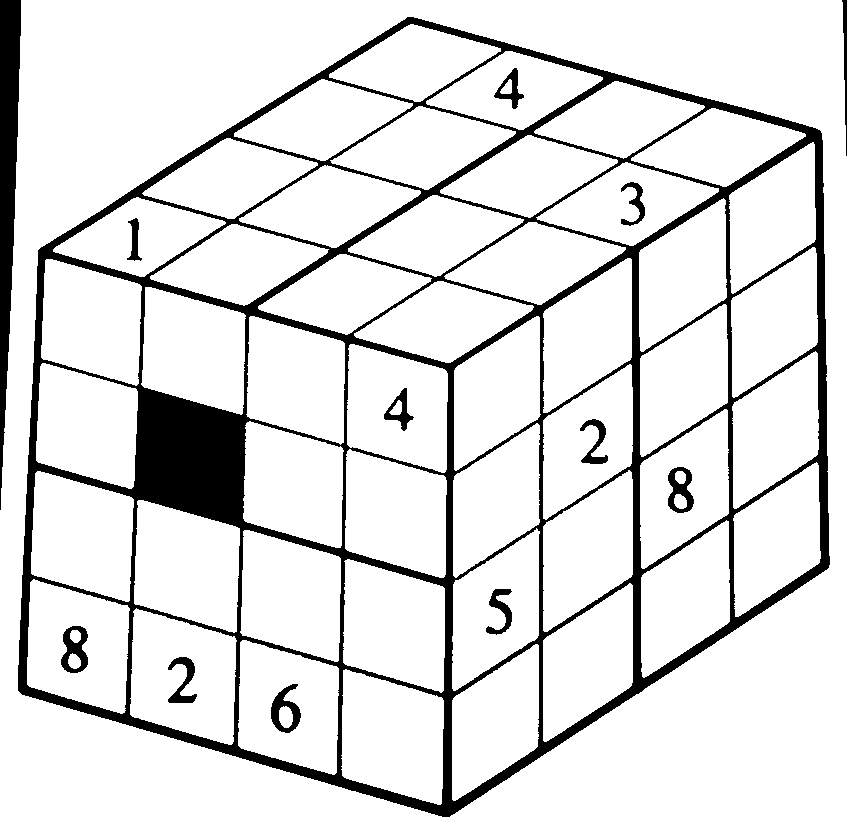
\includegraphics[scale=0.25]{fig/sudocubeThreshold.png}
\caption{Figure présentant un sudocube traité afin d'extraire les informations des cases}
\label{fig:sudoThresh}
\end{figure}

\begin{figure}[htbp]
\centering
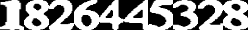
\includegraphics[scale=0.9]{fig/chiffresLues.png}
\caption{Figure présentant un exemple d'images extraites des cases du sudocube et normalisées avant d'être passées au lecteur de chiffres}
\label{fig:chifLu}
\end{figure}

\subsection{Les solutions retenus/considérés}
Pour le lecteur de chiffres, deux solutions furent considérées : la librairie Tesseract et l'algorithme d'intelligence artificielle KNearest implanté dans la librairie OpenCV. Tesseract est une librairie qui permet de faire la lecture de caractères de plusieurs langues. Cette solution offre des fonctionnalités non nécessaires en plus d'imposer une dépendance supplémentaire au projet. Puisqu’OpenCV est une dépendance obligatoire et que la méthode KNearest permet d'obtenir le même résultat qu'avec Tesseract le choix s'est arrêté sur cette première solution.

\subsection{Les moyens utilisé pour configurer}
L'extracteur de sudocube fut configuré (seuils, coefficients de dilatation et d'érosion) à partir d'un lot de tests de 42 images (angles, distances sudocube/robot et luminosités variées). La configuration fut réalisée par essais/erreur pour trouver les paramètres optimaux pour toutes les images.

Le lecteur de chiffres est entraîné avec 40 échantillons par chiffres. Puis, il est testé avec un lot de 60 nouvelles images par chiffres afin de vérifier sa robustesse.

\section{Solveur de Sudocubes}

\subsection{Composantes du solveur}
L'algorithme de résolution des sudocubes a été conçu en C++. L'emploi de la programmation par contraintes (CSP) aurait été  plus simple à implanter, mais cette solution n'a pas été envisagée au départ. Un prototype conçu en C++ était déjà réalisé au moment de la prise de conscience de l'existence de ce type de programmation. Le développement du solveur est actuellement terminé et ce dernier est fonctionnel.


\paragraph{}L'algoritmne utilise une structure de données afin de garder en mémoire le sudocube qui est représenté par un tableau à trois dimensions. La structure devient donc une interface pour la vision et permet de stocker les données obtenues lors de l'extraction du sudocube.
Les stratégies utilisées pour résoudre le sudocube sont les mêmes que celles  utilisées dans le monde des sudokus conventionnels, mais adaptées aux sudocubes. Elles sont présentées dans la liste suivante (ici citées en anglais pour les retrouver plus facilement sur Internet):\newline
\begin{itemize}
\item Naked pairs
\item Hidden pairs/triples
\item Pointing pairs/triples
\item Box and line reduction
\end{itemize}
\paragraph{}Si ces stratégies ne suffisent pas à résoudre le sudocube, la technique de force brute est employée. Il s'agit d'une solution acceptable puisque la probabilité d’occurrence de la situation est faible.

\paragraph{}L'algorithme peut trouver une solution à des sudocubes ayant uniquement 4 chiffres au départ. Il satisfait donc les exigences du client étant donné que les sudocubes présentés au laboratoires ont entre 9 et 14 chiffres. Le temps d'exécution varie de quelques millisecondes à quelques dizaines de millisecondes pour les sudocubes testés.

\subsection{Stratégie de test}
Pour tester entièrement notre classe solveur, il faudrait tester chacune des stratégies utilisées unitairement. Toutefois, tester chacune des stratégies requiert une architecture différente, puisque ces stratégies sont des méthodes privées de la classe solveur. Trois solutions sont envisageables:

Premièrement, il est possible de briser l'encapsulation de la classe solveur, ce qui n'est généralement pas une bonne pratique.

Sinon, un nouvel objet duquel hériterait chacune des stratégies peut être créé. De cette façon, les stratégies deviendraient des objets et seraient injectées dans la classe solveur à sa construction, préservant l'encapsulation. On aurait donc l'avantage de pouvoir tester chacune des stratégies unitairement, en plus de pouvoir isoler la classe solveur pour la tester (en utilisant des mocks). Cette façon de procéder correspond en fait au patron de conception "strategy". Cette façon de tester est la meilleure des trois côté qualité de code.

Finalement, l'encapsulation peut être préservée en ne testant tout simplement pas chacune des stratégies. Nous testerions uniquement la méthode "solve" en passant au solveur des sudocubes et en observant le résultat, ce qui ressemble plus à un test d'intégration.

Dans le cas de ce projet, la troisième option est employée puisqu'elle est plus simple et couvre suffisamment les différents cas du solveur. Ce test est un bon compromis entre le respect du bris d'encapsulation et le fait de tester unitairement chacune des stratégies. La deuxième stratégie serait plus complète, mais requiert trop de temps à implanter.

\section{Recherche de chemin}
La fonctionnalité recherche de chemin n’en est encore qu’au stade du prototype. La solution développée dans le prototype est viable, mais il reste du travail à faire pour qu'elle soit fonctionnelle. Il faudra entre autres ajouter une couche logicielle afin de réduire le nombre de points dans le chemin trouvé et ainsi réduire le nombre de rotations du robot.

\section{Communication microcontrôleur - Mac mini}

La communication entre le Mac mini a été réalisée avec un port série UART avec le protocole RS-232 à travers le module ICDI du microcontrôleur LM3S9B92. Ce protocole a été choisi en raison de sa simplicité et de la facilité du déverminage par rapport au protocole USB plus complexe. Une interface de communication qui passe des commandes sous forme de caractères a été développée du côté microcontrôleur. Un terminal série écrit en Python et utilisant la librairie Pyserial a été développé du côté ordinateur. Ce terminal pour usage diagnostique est compatible avec Linux et Windows et permet de récolter des données utiles sous forme de fichiers CSV pour le développement et les tests d'asservissement et de décodage d'antenne. Le terminal final aura une forme légèrement différente afin de s'interfacer avec ROS.

\section{Décodage du signal Manchester - partie logicielle}

Le décodage logiciel du signal de l'antenne doit transformer les bits en encodage Manchester en bits traditionnels. La méthode choisie doit être robuste aux changements de taux de transmission de bits, car il est spécifié dans la description du projet que ce taux peut varier de plus ou moins 50 bits / seconde. Parmis les algorithmes permettant de détecter des signaux de taux de transmission inconnu, il en existe deux types principaux : 

\begin{enumerate}
\item{Les algorithmes basés sur l'échantillonnage}

On effectue une mesure du signal à un intervalle prédéfini plus petit que la période du signal mesuré. C'est le décompte des bits consécutifs à zéro et à un qui permet de décoder le signal.

\item{Les algorithmes basés sur les timings} 

On effectue une mesure du temps entre les transitions du signal de zéro à un et de un à zéro. C'est le temps entre les montées et descentes qui permet de décoder le signal.
\end{enumerate}

Puisque le LM3S9B92 possède des compteurs d'usage général qui implémentent une fonction de capture d'événement, la méthode par timings a été employée. Ces compteurs peuvent être utilisés avec un canal du DMA du microcontrôleur. Les interruptions générées par les transitions déclenchent des transferts DMA vers un tampon de données qui contient les valeurs du compteur lors des interruptions. Les timings sont obtenus en soustrayant la valeur courante de la valeur précédente dans le tampon (le compteur est décrémental). 

La capture d'événements a d'abord été testée avec un signal PWM interne au microcontrôleur, puis des échantillons ont été pris avec le signal du récepteur d'antenne pour évaluer la variabilité du signal et pour tester notre algorithme de décodage. 

L'algorithme de décodage comporte trois étapes principales. 

Premièrement, on recherche le plus petit timing qui n'est pas un artéfact. Étant donné la façon dont le circuit du récepteur est conçu, ce timing correspond à un zéro simple, puisque que les montées sont plus rapides que les descentes. Ce timing permet d'avoir une référence pour les valeurs à zéro et permet d'attribuer une valeur de 0 ou 1 à chaque timing, sachant qu'elles alternent. En parcourant les valeurs à un, il est ensuite possible d'obtenir une référence similaire pour les valeurs à 1.

Ensuite, les données brutes sont traitées pour enlever les artéfacts et assigner à chaque timing une valeur de '0' simple, '1' simple, deux '0' consécutifs ou deux '1' consécutifs. Ceci est possible grâce aux références pour les 0 et les 1 qui permettent de déterminer un seuil pour assigner une valeur double plutôt que simple.

Finalement, un algorithme de recherche de séquences tel l'algorithme de Knuth-Morris-Pratt peut être utilisé pour trouver la séquence des bits d'arrêt et de départ afin de trouver le point de départ et décoder le signal utile.

\section{Orientation du robot}

Pour la détermination de l'angle d’orientation du robot, le choix de la caméra embarquée offre une meilleure précision que celui de la Kinect. 

\paragraph{}Dans un premier temps, la caméra doit être calibrée. Pour ce faire, deux méthodes sont envisageables: soit l’application de l’algorithme de Zhang ou la calibration avec OpenCV. La méthode retenue est celle employant l'algorithme de Zhang, car elle est plus efficace. 

\paragraph{}Ensuite, la détermination de l’angle du robot par rapport à la ligne rouge présente sur la table est réalisée avec un traitement d’image supportant la variation de luminosité, d’ombres, ainsi qu'au moyen de règles de trigonométrie.

\paragraph{}Enfin, la détermination de l’orientation du robot (N, S, E, O) est effectuée en détectant les coins de la table. 
L’algorithme de cette opération est assez simple. Si la caméra détecte le coin orange avant le bleu, le robot sera orienté vers le Nord. Si elle détecte le coin bleu avant le coin orange, le robot sera orienté au Sud. La détection des deux coins bleus montrera une orientation vers l’Ouest et enfin la détection des deux coins orange montrera une orientation vers l’Est.

\paragraph{}Les deux dernières parties sont commencées, mais ne sont pas encore complétées à ce jour.


\section{Vision par Kinect}
Pour aider au déplacement du robot, la Kinect a été utilisée afin de détecter la position des obstacles, la position du robot lui-même ainsi que sa position angulaire par rapport au point (0.0) de notre représentation cartésienne de la table. Toutefois, comme la Kinect est située à l'extérieur de la table de jeu, il faut une translation et une rotation des données obtenues afin de positionner les objets avec exactitude. Les 3 sections qui suivent expliquent en détail les différentes parties de l'algorithme de vision de la Kinect.

\subsection{Transformation des distances}
En premier lieu, il est important de clarifier quelles distances il est possible d'obtenir à l'aide de la Kinect. Le «Framework» OpenNI est capable de retourner 2 types de distances pour chacun des points dans l'image infrarouge obtenue de la Kinect. Le premier type de distances retourné est la longueur, en mètres, entre l'objectif et un point quelconque sur l'image. Le second type est dérivé du premier et correspond aux composantes X, Y et Z du vecteur de longueur entre l'objectif et la cible. Pour aider à la compréhension, les deux types de distances peuvent être représentés par les lignes vertes sur l'image \ref{fig:kinect_distance}. Toutefois, comme l'origine de notre représentation cartésienne de la table est situé sur le coin inférieur droit de la table et que la Kinect n'est pas située à cet endroit, il est nécessaire d'obtenir la distance X et Y (lignes bleues sur l'image \ref{fig:kinect_distance}) entre l'origine et le point ciblé sur l'image obtenue de la Kinect. Pour y arriver, il suffit d'obtenir la position X et Y (lignes rouges sur l'image \ref{fig:kinect_distance}) de la lentille infrarouge de la Kinect ainsi que l'angle de la Kinect avec l'axe X de la table. Avec ces valeurs, dans notre cas 14cm, -56cm et $23.5^o$, un logiciel a été mis en oeuvre pour permettre la transformation des distances de la Kinect vers les composantes X et Y recherchées à l'aide de règles de trigonométrie simples. Cet algorithme possède une précision de plus ou moins 1cm pour n'importe quel point situé sur l'image obtenue avec la Kinect. 

\begin{figure}[htbp]
\centering
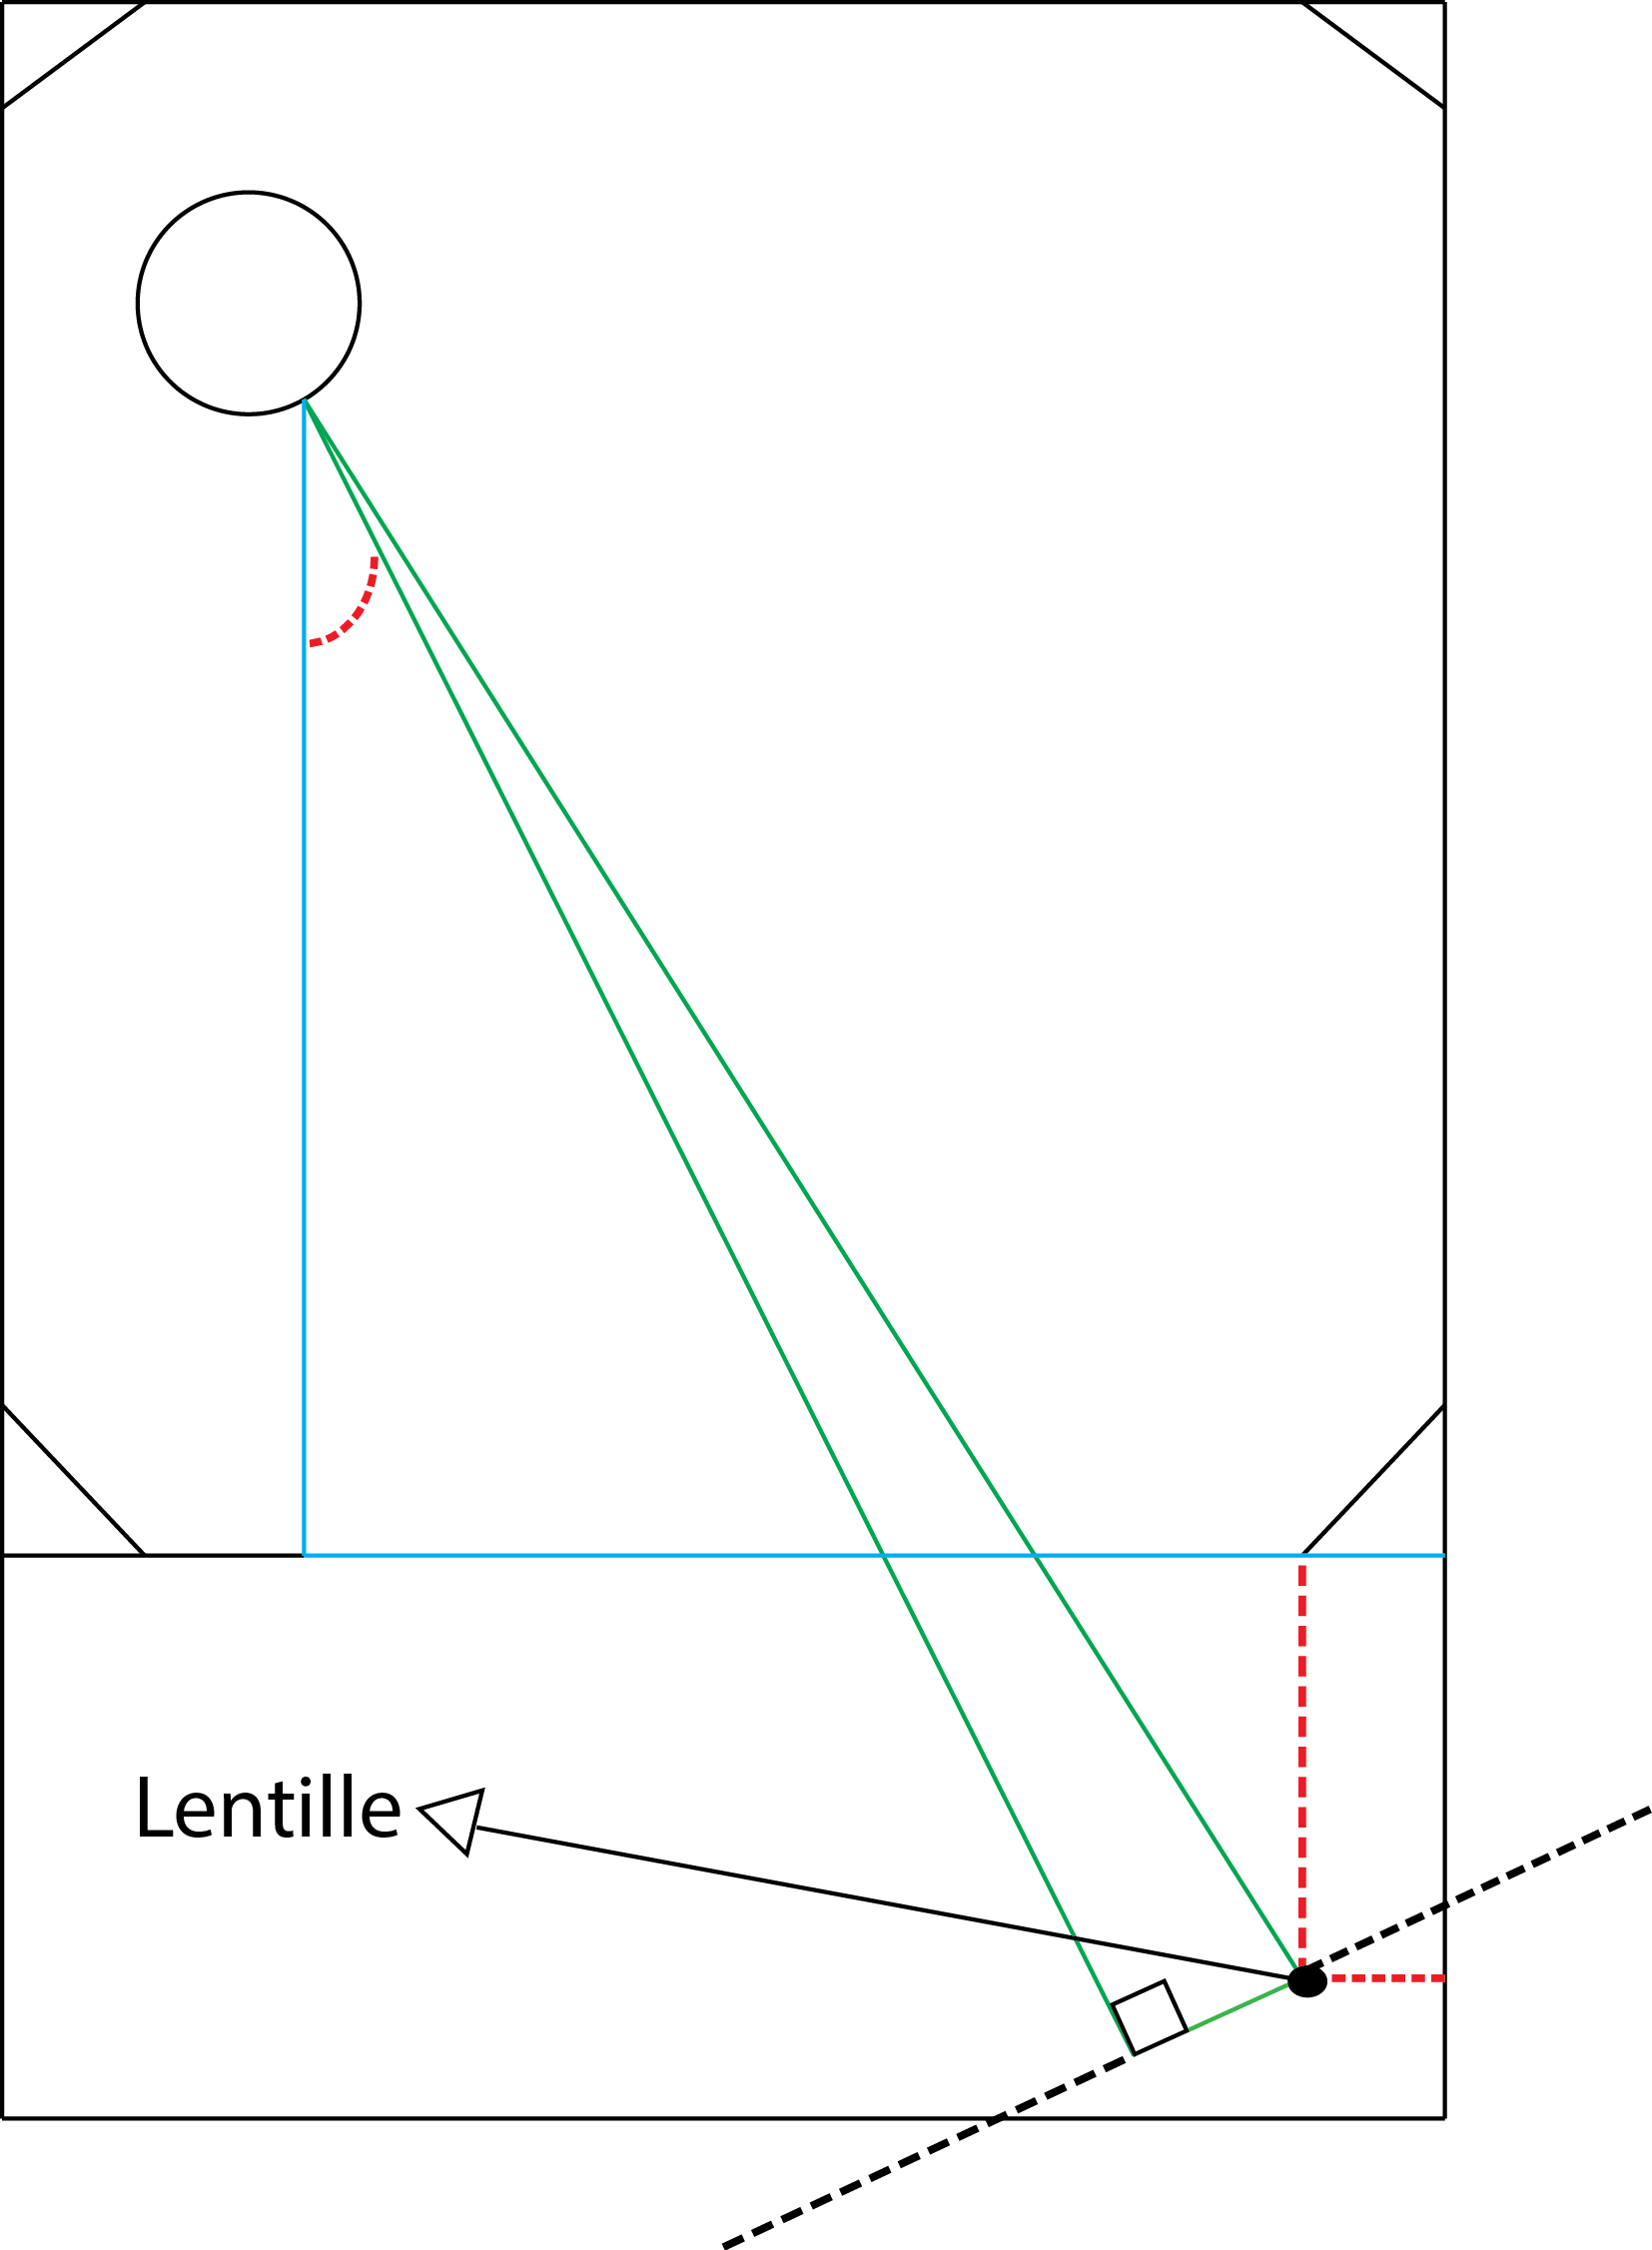
\includegraphics[scale=0.5]{fig/kinect_distance.png}
\caption{Schéma représentant la table et les différentes mesures obtenues avec la Kinect pour un point quelconque}
\label{fig:kinect_distance}
\end{figure}

\subsection{Détection des obstacles}
Comme il est possible d'obtenir n'importe quelle distance entre l'origine et un point quelconque sur l'image, un algorithme de recherche d'obstacles a été créé. Sachant que les obstacles sont situés dans une zone précise sur la table et que ceux-ci font 40cm de hauteur, il suffit de rechercher tout objet de cette hauteur situé dans la zone prédéfinie. La Kinect retourne la hauteur de chacun des points sur l'image infrarouge et permet de localiser les obstacles. De plus, à l'aide de calculs statistiques, l'algorithme est en mesure de trouver les obstacles lorsqu'ils sont presque alignés ou obstrués par un autre objet comme le robot. Comme cet algorithme dépend entièrement de l'algorithme précédent, les positions obtenues pour chacun des obstacles possèdent la même incertitude de 1 cm sur chaque mesure de distance effectuée. En ce qui concerne l'efficacité de l'algorithme, différents tests montrent un temps de calcul d'environ 30 ms sur un Core 2 Duo 2.4 GHz pour obtenir la position du centre des deux obstacles.

\subsection{Détection du robot}
En ce qui concerne la détection du robot, un algorithme semblable à la détection des obstacles à été utilisé. Comme le robot possède une hauteur d'environ 20cm et une profondeur semblable, il est possible d'isoler, dans la matrice de distance, un carré qui correspond aux dimensions du robot. De plus, la précision de la détection du robot peut être améliorée par la mise en place d'une recherche de symboles de couleur spécifique sur le robot à l'aide de la caméra RGB de la Kinect. Avec cette méthode qui n'est pas encore implémentée, il sera possible d'obtenir la position réelle du robot, peu importe sa position sur la table, et ce avec une vitesse qui se rapproche de l'algorithme de détection des obstacles. Pour le moment, en se servant seulement de la détection par contrainte de distance, il est possible de détecter le robot avec une incertitude de 5 cm en environ 30 ms si le robot n'est pas situé derrière un obstacle.

\section{Communication entre le Mac mini et la station de base}
\subsection{Composantes du système}
Avant de pouvoir communiquer avec le robot, l’adresse IP du robot est récupérée grâce à un script bash exécuté lors du démarrage de celui-ci. Le script récupère l’adresse IP et l’envoie par courriel à un compte gmail.

Ensuite, ROS est employé pour gérer la communication entre les différents nodes ROS. Un node est une application qui utilise l’API de ROS. Actuellement, l’envoi de messages au Mac mini pour démarrer la séquence du robot a été testé.

Le diagramme \ref{fig:commNodes} présente la répartition des nodes sur les différents appareils ainsi que les appareils avec lesquels chaque node travaille. Le node du Mac mini est séparé en deux en deux afin de simplifier les tests pour les composantes qui communiquent avec le microcontrôleur. Grâce au système de communication de ROS, il est possible d'envoyer, par ligne de commande, des messages afin de déplacer le robot ou encore d'afficher un message sur l’écran LCD, et ce, sans passer par l’écriture d’une application de tests.

\begin{figure}[htbp]
\centering
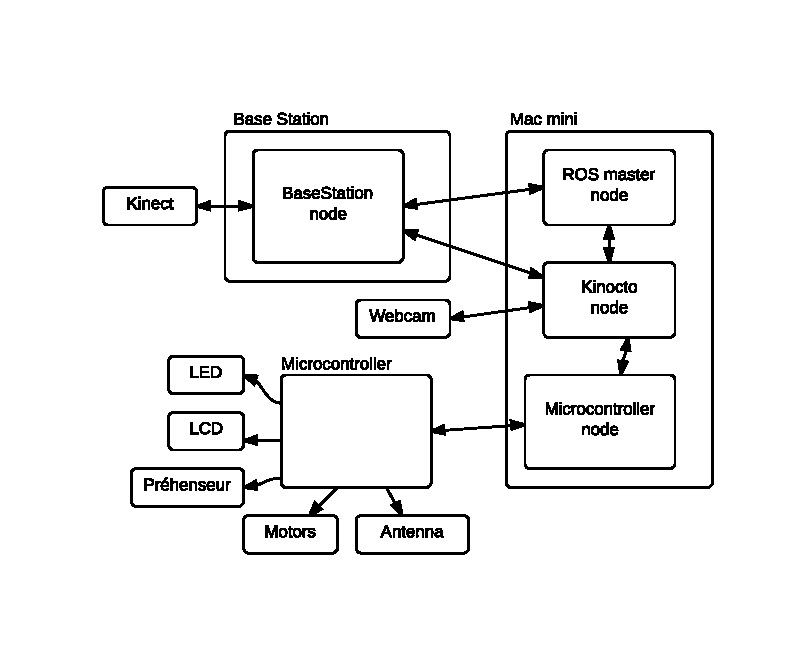
\includegraphics[scale=1]{fig/communicationNodesAppareils.pdf}
\caption{Diagramme représentant la communication entre les nodes et les différents appareils}
\label{fig:commNodes}
\end{figure}

\subsection{Les solutions retenues et considérées}
Deux solutions ont été considérées : POCO, une librairie C++, et ROS, un environnement de développement pour robot.

\paragraph{}POCO permet d’envoyer des chaînes de caractères par TCP/IP. L’envoie de commandes avec POCO consiste en ces étapes : concaténer le nom d’une commande (choisit au préalable) et ses arguments dans une chaîne de caractères. Puis, envoyer, à l’aide de la librairie, la chaîne de caractères. Il faut extraire la commande et ses paramètres lors de la réception d’un message.

\paragraph{}ROS fait exactement la même chose que POCO en arrière-plan, mais il y a une couche logicielle qui donne des avantages supplémentaires. Pour envoyer des messages entre deux applications ROS, iI suffit de déclarer, pour chaque type de message, des variables et leur type dans un fichier texte. Puis, lors de la compilation, le projet ROS génère des struct en C pour chaque message. Ensuite, l’api de ROS est employée pour définir le contenu des messages et envoyer les messages.

\paragraph{}La courbe d’apprentissage est plus prononcée avec ROS. Cependant, avec celui-ci les messages sont hachés avec une somme MD5 et lorsqu’un message est reçu par une node (une application ROS) le contenu est vérifié avec la somme MD5, nous garantissant ainsi que le message s’est transmis.

\paragraph{}De plus, il est possible d’enregistrer tous les messages qui sont envoyés par ROS depuis le démarrage de la séquence, de les consulter séquentiellement dans le temps grâce à une interface graphique et de les exécuter à nouveau afin de reproduire la même séquence de message. C’est un outil de déverminage qui sera utile lors du développement de l’agent intelligent et que l’on ne possède pas avec POCO.

ROS a été retenu pour ses nombreux avantages. 
